\documentclass[11pt]{article}

\usepackage{amsmath}
\usepackage{amsfonts}
\usepackage{amssymb}

% Give ourself extra space for text
\usepackage[left = 2.2cm, right = 2.2cm, top = 1.8cm, bottom = 2.8cm]{geometry}

% Allows us to easily change the numbering system used in things like \begin{enumerate}. https://ctan.org/tex-archive/macros/latex/contrib/enumitem/
\usepackage[shortlabels]{enumitem}

% Turns table of contents, \refs, etc. into hyperlinks
\usepackage{hyperref}

% To include image, just use \includegraphics[scale=•]{relative path to image}
\usepackage{graphicx}
\graphicspath{ {./images/} }

% Common sets
\newcommand{\integers}{\mathbb{Z}}
\newcommand{\naturals}{\mathbb{N}}
\newcommand{\reals}{\mathbb{R}}

% Power set
\newcommand{\powerset}{\mathcal{P}}

% Identity matrix
\newcommand{\ident}{\mathbb{I}}

% Inverse hyperbolic functions
\DeclareMathOperator{\arcosh}{arcosh}
\DeclareMathOperator{\arsinh}{arsinh}
\DeclareMathOperator{\artanh}{artanh}

% I hat, J hat, K hat
\newcommand{\ihat}{\boldsymbol{\hat{\textbf{\i}}}}
\newcommand{\jhat}{\boldsymbol{\hat{\textbf{\j}}}}
\newcommand{\khat}{\boldsymbol{\hat{\textbf{k}}}}

% Better vectors (for single characters)
\renewcommand{\vec}[1]{\mathbf{#1}}

% Allows us to number equations in \begin{align} statements, etc.
\newcommand\numberthis{\addtocounter{equation}{1}\tag{\theequation}}

% Augmented matrices: this allows us to make augmented matrics using something like \begin{bmatrix}[cc|c]. Taken from Stefan Kottwitz at https://tex.stackexchange.com/questions/2233/whats-the-best-way-make-an-augmented-coefficient-matrix.
\makeatletter
\renewcommand*\env@matrix[1][*\c@MaxMatrixCols c]{%
  \hskip -\arraycolsep
  \let\@ifnextchar\new@ifnextchar
  \array{#1}}
\makeatother

% NOTE: This means \section does NOT number sections, but ensures that they appear in the table of contents, which does not occur if simply \section* is used. From egreg @ https://tex.stackexchange.com/a/30225.
\setcounter{secnumdepth}{0} % sections are level 1

\begin{document}
\title{ENG1005: Lecture 25}
\author{Lex Gallon}
\maketitle

\tableofcontents

\section*{Video link}
\url{https://echo360.org.au/lesson/G_8402119b-734b-4e1e-a3b4-7e907e86ddba_b944cecf-8ba5-40d3-a870-0243a0a9e78c_2020-05-19T15:58:00.000_2020-05-19T16:53:00.000/classroom#sortDirection=desc}

\subsubsection{Example}
Estimate the change in the period
\[ T = 2\pi \sqrt{\frac{L}{g}} \]
of a simple pendulum due to a 2\% increase in length $L$ and a 0.6\% decrease in the gravitational acceleration $g$.

\subsubsection{Solution}
\[ dL = \frac{2}{100}L \text{ and } dg = \frac{-6}{1000}g \]
Substituting this into
\begin{align*}
dT &= \frac{\partial T}{\partial L}\, dL + \frac{\partial T}{\partial g}\, dg \\
&= 2\pi \frac{1}{2 \sqrt{\frac{L}{g}}} \frac{1}{g}\, dL + 2\pi \frac{1}{2 \sqrt{\frac{L}{g}}} \left( \frac{-L}{g^2} \right)\, dg \\
&= \frac{\pi}{\sqrt{Lg}}\, dL - \frac{\pi \sqrt{L}}{g^{\frac{3}{2}}}\, dg 
\end{align*}
yields
\begin{align*}
dT &= \frac{\pi}{\sqrt{Lg}} \frac{2}{100}L + \frac{\pi \sqrt{L}}{g^{\frac{3}{2}}} \frac{6}{1000}g \\
&= \frac{2\pi}{100} \sqrt{\frac{L}{g}} + \frac{6 \pi}{1000} \sqrt{\frac{L}{g}} \\
&=  \frac{26\pi}{1000} \sqrt{\frac{L}{g}} \\
&= \frac{13}{1000} T
\end{align*}

So there is a 1.3\% increase in the period of a pendulum.

\section{Tangent plane}
Given a function $f(x,y)$, then the curves
\[ \vec{r}(s) = (a+s, b, f(a+s, b));\quad \vec{r}(0) = (a, b, f(a, b)) \]
\[ \vec{\tilde{r}}(t) = (a, b + t, f(a, b+t));\quad \vec{\tilde{r}}(0) = (a, b, f(a, b)) \]
lie on the graph
\[ S = \{ (x, y, f(x, y)) | (x, y) \in D \} \subset \reals^3 \]
and pass through the point $p = (a, b, f(a,b))$ at $s=0$ and $t=0$, respectively.

\begin{align*}
\frac{d\vec{r}}{dS}(0) &= \left. \frac{d}{ds} ((a+s, b, f(a+s, b)) \right|_{s=0} \\
&= \left. \left( 1, 0, \frac{\partial f}{\partial x}(a+s, b) \frac{d}{ds}(a+s) \right) \right|_{s=0} \\
&= \left( 1, 0, \frac{\partial f}{\partial x}(a, b) \right)
\end{align*}

\begin{align*}
\frac{d\vec{\tilde{r}}}{0} &= \left. \frac{d}{dt}(a, b+t, f(a, b+t)) \right|_{t=0} \\
&= \left( 0, 1, \frac{\partial f}{\partial y}(a, b) \right)
\end{align*}

\subsection{Tangent plane parametrisation}
\begin{align*}
\vec{\ell} &= \vec{p} + h \frac{d \vec{r}}{ds}(0) + k \frac{d\vec{\tilde{r}}}{dt}(0) \\
&= (a, b, f(a, b)) + h \left( 1, 0, \frac{\partial f}{\partial x}(a, b) \right) + k \left( 0, 1, \frac{\partial f}{\partial y}(a, b) \right) \\
\Rightarrow \ell(h, k) &= \left(a+h, b + k, f(a, b) + \frac{\partial f}{\partial x}(a, b) h + \frac{\partial f}{\partial y}(a, b) k \right)
\end{align*}

Setting
\[ h = x-a \text{ and } k = y-b \]
gives
\[ \ell(x, y) = \left(x, y, f(a, b) + \frac{\partial f}{\partial x}(a, b) (x-a) + \frac{\partial f}{\partial y}(a, b) (y-b) \right) \]

So this has now given us a \textbf{parametrisation of the tangent plane} to the graph of $S$ of $f(x,y)$ at the point $(a, b, f(a,b))$.

But note that the tangent plane is the graph of the linearisation of $f(x,y)$! This makes sense really since, when we're linearising, we take the first order terms around a given point, which seems analogous to taking the first order derivative of a line in $\reals^2$ (which gives the tangent line.

\section{Maximum and minimum values §9.7.2, 9.7.3}
\subsection{Definition}
A function $f(x,y)$ has a
\begin{enumerate}[ (i) ]
\item local maximum at $(a, b)$ if there exists some $R > 0$ such that $f(x, y) \leq f(a, b)$ for all $(x, y) \in B_R ((a, b))$.
\item local minimum at $(a, b)$ if there exists some $R > 0$ such that $f(x, y) \geq f(a, b)$ for all $(x, y) \in B_R ((a, b))$.
\item absolute maximum at $(a ,b)$ if $f(x,y) \leq f(a, b)
$ for all $(x, y) \in D$ (where $D$ is the domain of $f$).
\item absolute minimum at $(a ,b)$ if $f(x,y) \geq f(a, b)$ for all $(x, y) \in D$ (where $D$ is the domain of $f$).
\end{enumerate}

\subsection{Definition}
A point $(a, b) \in \reals^2$ is called a critical (stationary) point of $f(x, y)$ if $\nabla f(x, y) = \vec{0}$ or $\nabla f(a, b)$ is undefined. (is that meant to be $x, y$ or $a, b$, not sure?)

\subsection{Theorem}
If the gradient $\nabla f(x, y)$ exists at $(a, b)$ and $(a, b)$ is either a local maximum or a local minimum of $f(x,y)$ then $\nabla f(a,b) = \vec{0}$.

\subsection{Definition}
If $(a, b)$ is a point such that $\nabla f(a, b) = \vec{0}$ but $(a, b)$ is neither a local minimum or a local maximum, then $(a, b)$ is called a saddle point.

\subsection{Examples}
\begin{enumerate}[ (i) ]
\item $f(x, y) = 1 - x^2 - y^2$.

\begin{align*}
\nabla f(x, y) &= (-2x, -2y) \\
\Rightarrow \nabla f(0, 0) &= (0, 0) \Rightarrow (0, 0) \text{ is a critical point }
\end{align*}
and if you look at the graph of $f(x, y) = 1 - x^2 - y^2$, we can see that $f(x, y)$ has an absolute maximum at $(0, 0)$.

\begin{center} 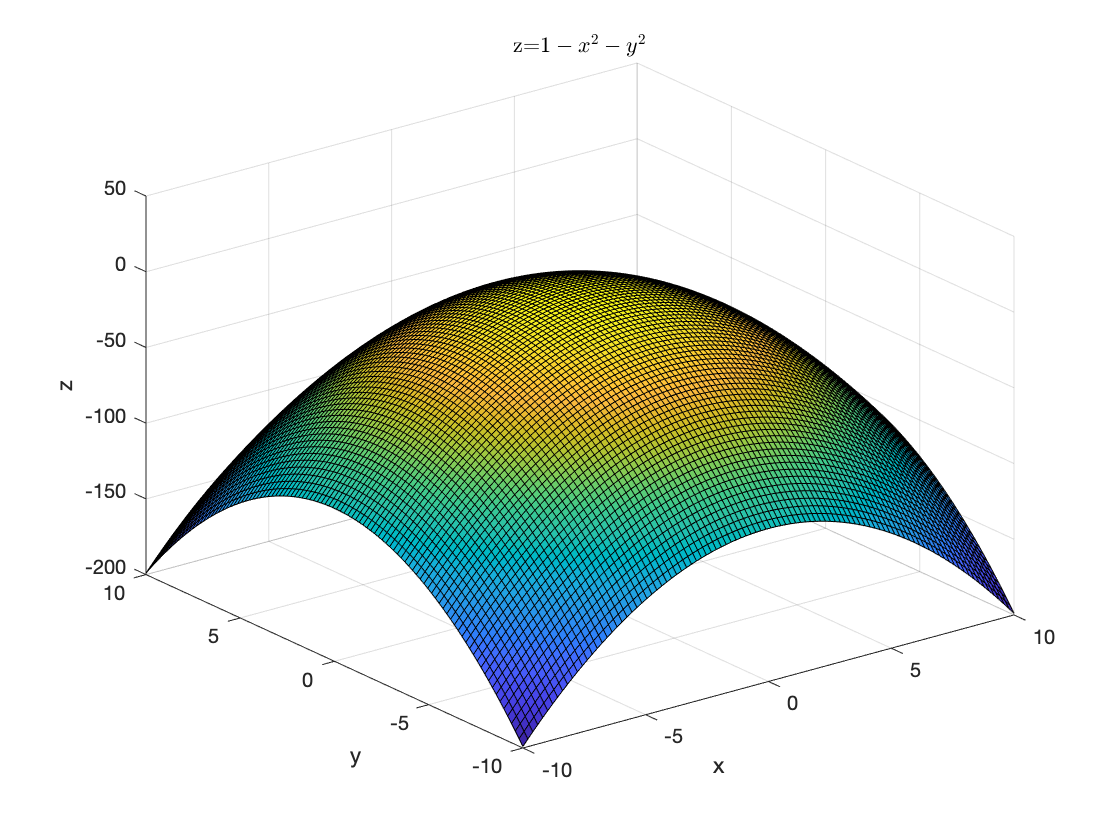
\includegraphics[scale=0.25]{eg1} \end{center}

\item $f(x, y) = x^2 + y^2$
\begin{align*}
\nabla f(x, y) &= (2x, 2y) \\
\nabla f(0, 0) &= (0, 0) \Rightarrow (0, 0) \text{ is a critical point}
\end{align*}
and we can similarly look at this graph to see that $f(x, y) = x^2 + y^2$ has an absolute minimum at $(0, 0)$.

\begin{center} 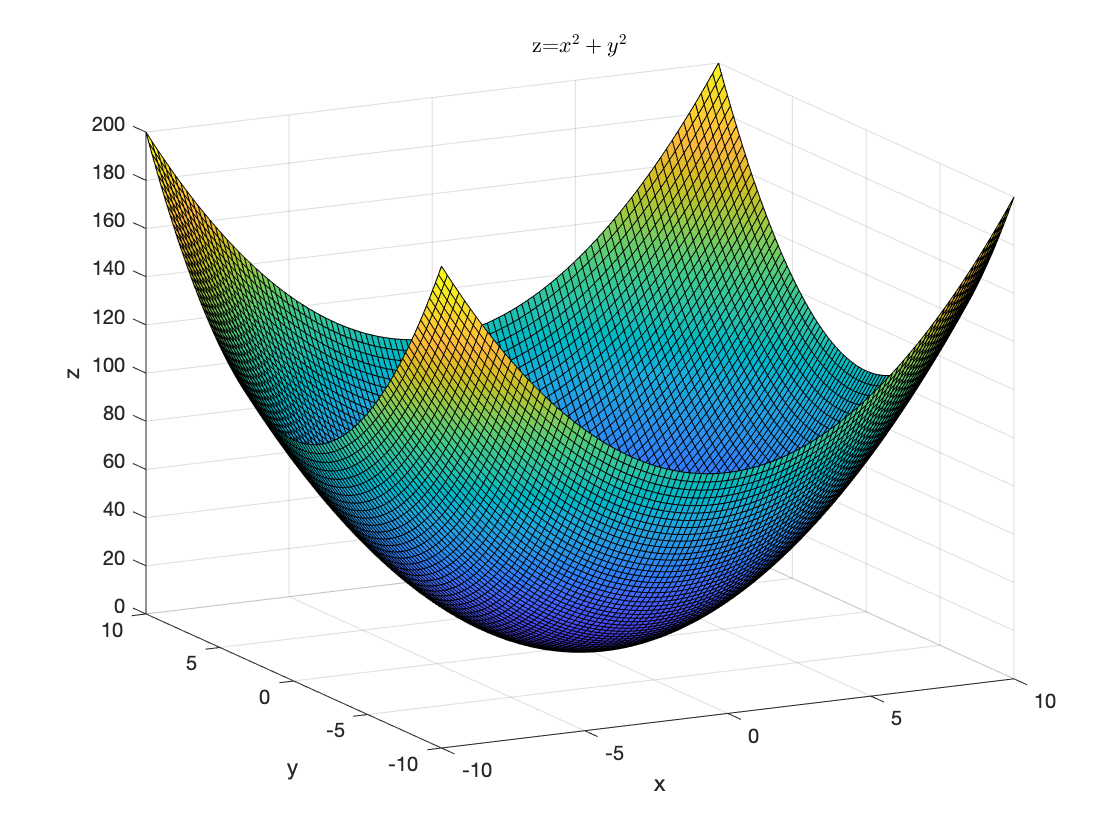
\includegraphics[scale=0.25]{eg2} \end{center}

\end{enumerate}

\end{document}